\section{Broader Small-Model Ecosystem Context}
\label{appendix:ecosystem}
\label{supp:last}

This appendix situates the reviewed \gls{slm} cohort within the wider model ecosystem, which matters because the 2025--2026 release cycle moved compact open models, open-weight reasoning models, and frontier API systems in parallel rather than in sequence. The summary below records the ecosystem context needed to interpret the cohort, followed by the full generated variant inventory.

\subsection{Landscape Snapshot}
\label{subsec:ecosystem_snapshot}
Three ecosystem trends are especially relevant to the present study:
\begin{description}
    \item[Capability compression] Reasoning, long-context handling, and multimodality have moved into the 1B--8B range, narrowing the gap between deployable \glspl{slm} and cloud-scale \glspl{llm}.
    \item[Open-weight expansion] Families such as Qwen, Phi, Gemma, SmolLM, DeepSeek distills, Granite, and MiniCPM have expanded the design space for self-hosted deployment (Figure~\ref{fig:license_posture}).
    \item[Deployment diversification] Inference targets now span cloud GPUs, consumer GPUs, laptops, smartphones, browsers, and embedded edge boards, making model choice inseparable from hardware choice.
    \item[The small-active-parameter turn] The most distinctive feature of the mid-2026 wave is how much of it activates 3--13B parameters against totals of 30B to 284B: Nemotron 3.5 Lightning (30B/3B), Hy-MT2-30B-A3B, North Mini Code (30B/3B), Laguna XS 2.1 (33B/3B), Ling 3.0 Flash (124B/5.1B) and its domain variants, and DeepSeek V4 Flash (284B/13B). These are the models that make the C1/C2 distinction load-bearing rather than pedantic, since each is cheap per token and none is resident on a phone.
\end{description}

The May--September 2026 additions to the inventory illustrate both ends of the range. At the small end, IBM shipped Granite 4.1 and then Granite 4.2 at 3B and 8B with a thinking switch, Liquid AI extended LFM2.5 from 230M to an 8.3B/1.5B on-device \gls{moe}, and Tencent released the Hy-MT2 translation family at 1.8B and 7B. Frontier API releases continued in parallel over the same months; they are recorded, with their sources, in the \gls{llm} part of the released inventory, and none of them bears on a claim in this paper.

Figure~\ref{fig:family_treemap} gives a size-proportional overview of the inventory by developer and family, and Figure~\ref{fig:developer_diversity} tracks the entry of new developers into the open-SLM space.

\begin{figure}[ht]
  \centering
  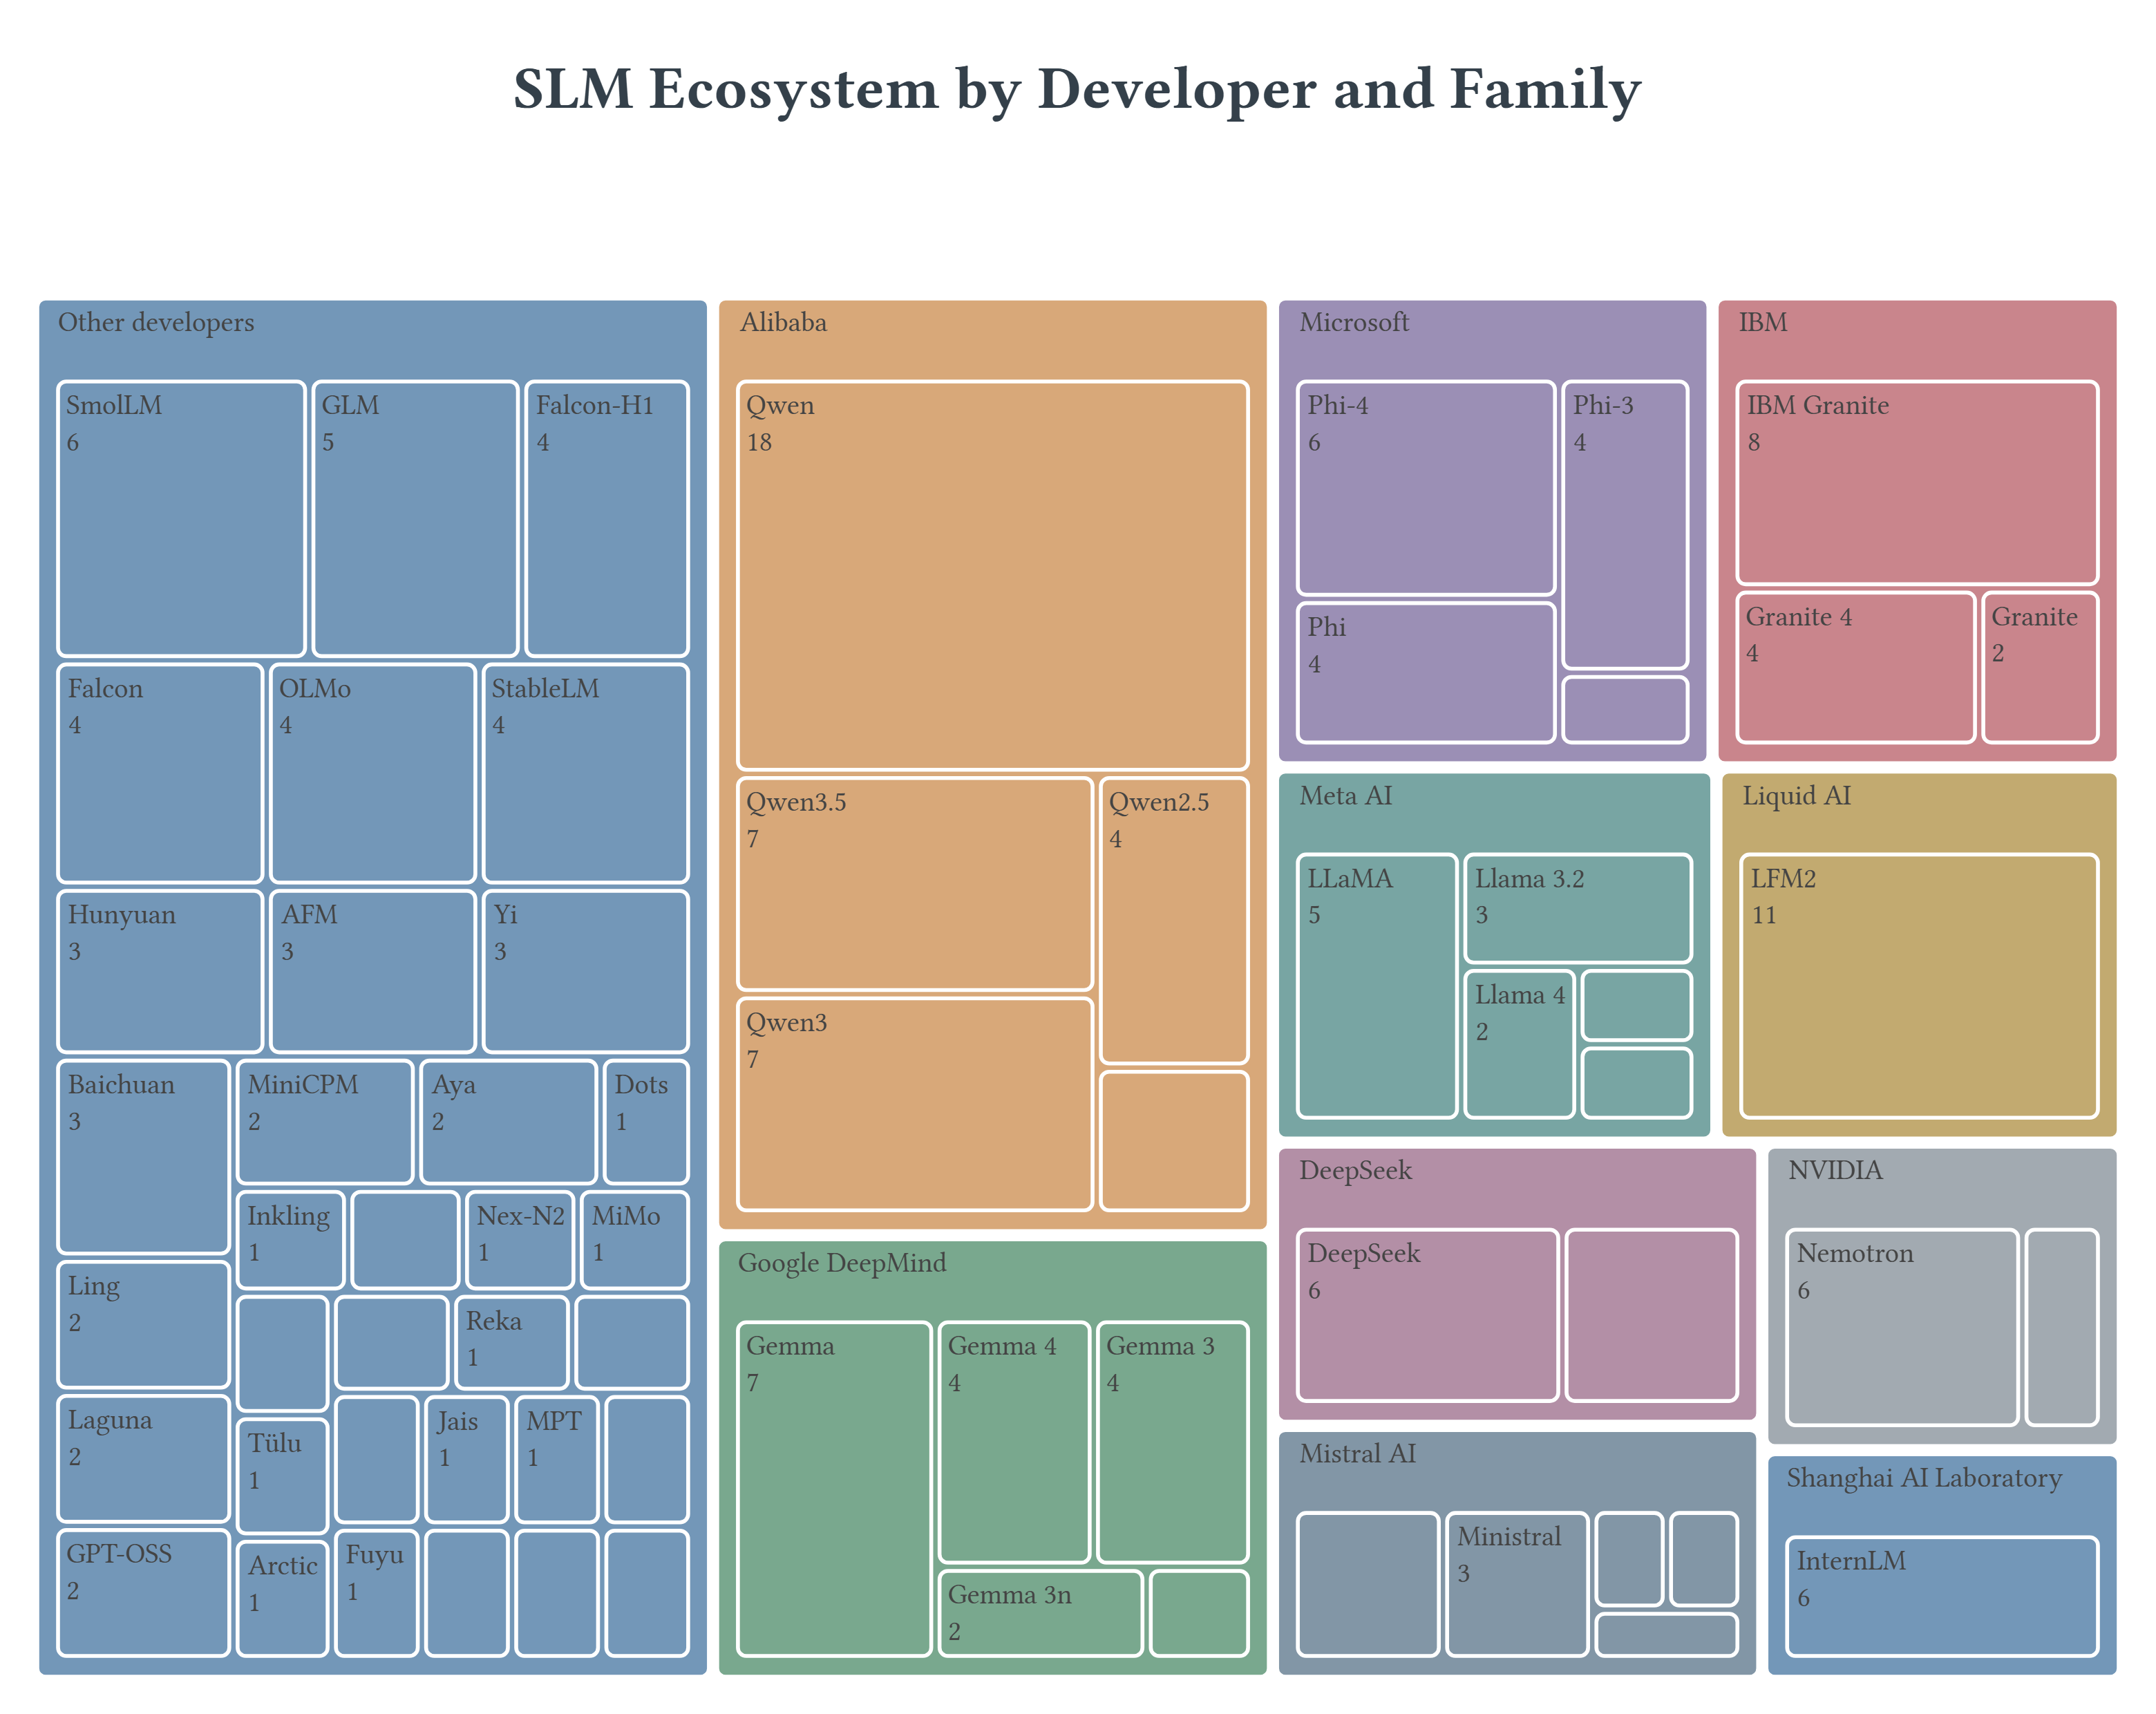
\includegraphics[width=\linewidth]{paper_slm_family_treemap.png}
  \caption{Documented SLM variants grouped by developer and family; area is proportional to the number of variants. Generated from \file{merged\_llm\_database.json} (version~3.6; releases through 4~September 2026).}
  \Description{Treemap of documented small language model variants grouped by developer and then by family, with rectangle area proportional to the number of variants in each group.}
  \label{fig:family_treemap}
\end{figure}

\begin{figure}[ht]
  \centering
  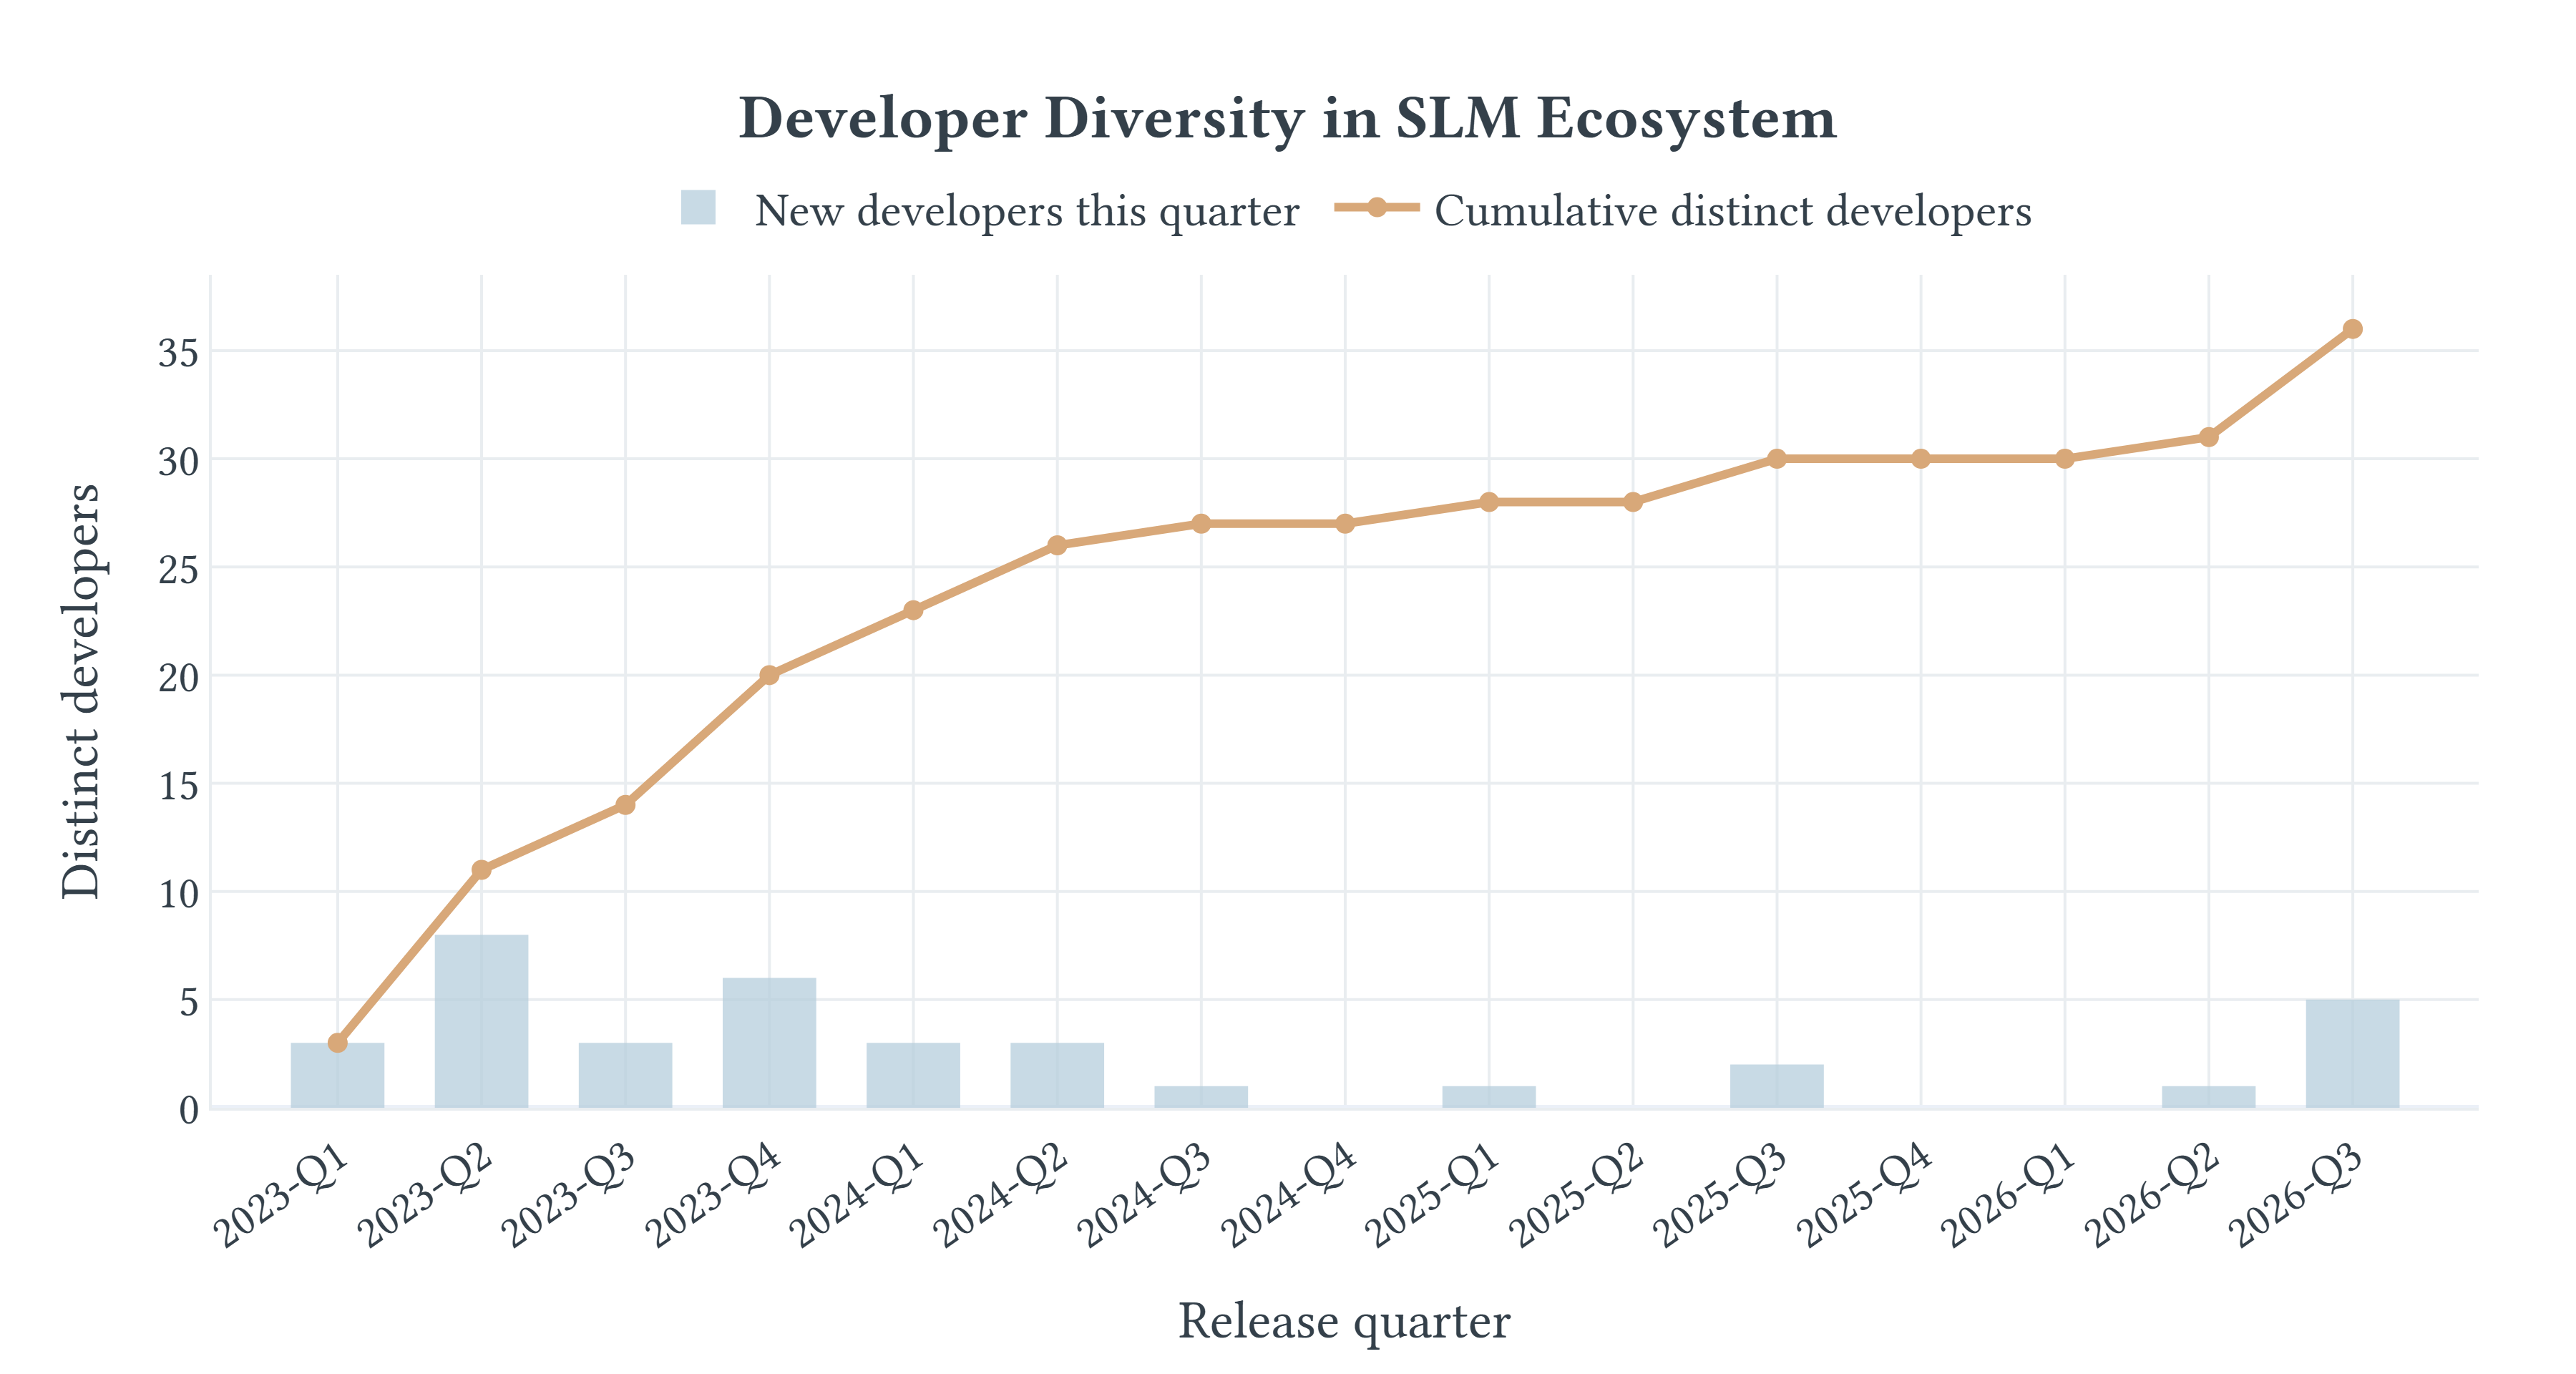
\includegraphics[width=\linewidth]{paper_slm_developer_diversity_timeline.png}
  \caption{Cumulative distinct developers releasing documented SLM variants (line) and new developers per quarter (bars).}
  \Description{Combination chart with bars showing the number of new developers releasing their first documented small language model in each quarter, overlaid with a line showing the cumulative count of distinct developers.}
  \label{fig:developer_diversity}
\end{figure}

\begin{figure}[ht]
  \centering
  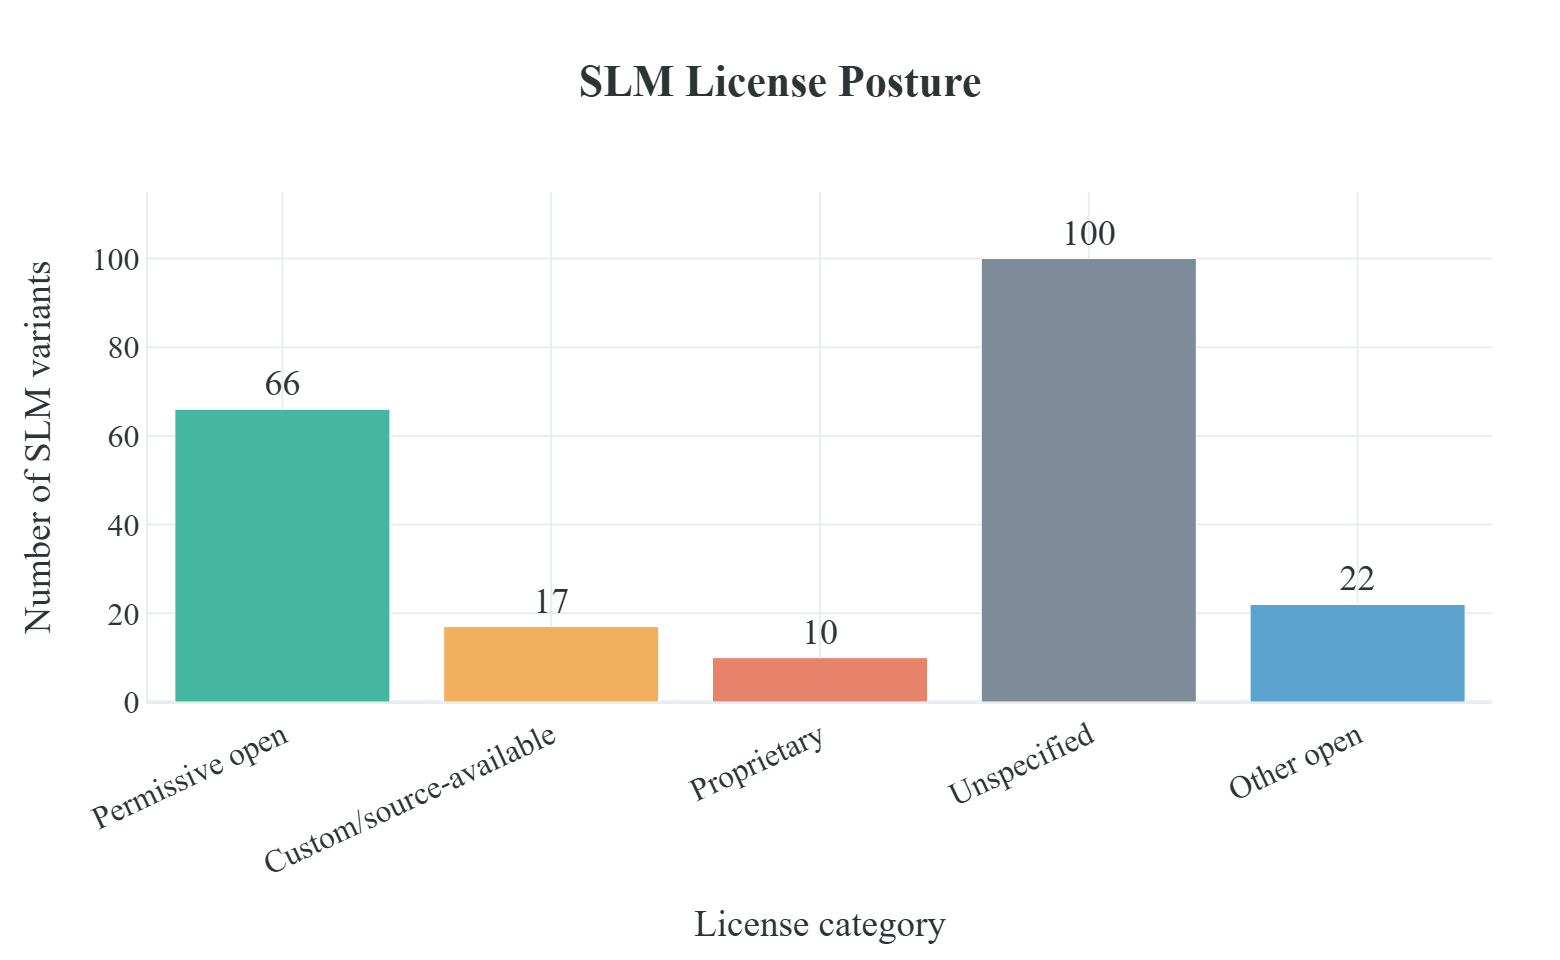
\includegraphics[width=0.78\linewidth]{paper_slm_license_posture.png}
  \caption{License posture of documented SLM variants. Permissive open licenses (Apache-2.0, MIT) account for the plurality; ``unspecified'' entries are typically research checkpoints without an attached license file.}
  \Description{Bar chart of documented small language model variants by license category. Permissive open licenses, chiefly Apache 2.0 and MIT, form the plurality, followed by custom vendor licenses and unspecified research checkpoints.}
  \label{fig:license_posture}
\end{figure}

\subsection{Representative Family Reference}
\label{subsec:ecosystem_families}
Table~\ref{tab:ecosystem_families} lists the representative families tracked in the inventory, with their developers, size ranges, access, and the role each plays in the landscape.

\begin{table}[ht]
\centering
\caption{Representative model families tracked in the inventory.}
\label{tab:ecosystem_families}
\footnotesize\adjustbox{max width=\linewidth}{%
\begin{tabular}{lllll}
\toprule
\textbf{Family} & \textbf{Developer} & \textbf{Representative Versions} & \textbf{Access} & \textbf{Typical Role} \\
\midrule
Qwen2.5 / Qwen3 & Alibaba & 0.5B--14B dense, MoE variants & Open weights & Strong multilingual, math, and code performance \\
Phi-3 / Phi-4 & Microsoft & 3.8B mini variants, 14B reasoning & Open weights & Data-curated reasoning-focused SLMs \\
Gemma 2 / 3 / 3n & Google DeepMind & 1B--12B dense, mobile-first multimodal variants & Open weights & Distilled compact models \\
Llama 3.2 / 4 & Meta & 1B--3B edge models, larger MoE frontier models & Open weights & Broad deployment ecosystem from edge to server \\
SmolLM2 / SmolLM3 & Hugging Face & 135M--3B & Open weights & Lightweight, fully open research and edge baselines \\
DeepSeek distills & DeepSeek & 1.5B--14B distilled reasoning models & Open weights & Reasoning transfer into self-hosted sizes \\
Granite 3 / 4 & IBM & 2--8B dense; 4.0 hybrid Mamba-2/MoE (350M--32B, 1--9B active) & Open weights & Enterprise-friendly, tool-use and RAG focus \\
Falcon-H1 & TII & 0.5--34B parallel attention/Mamba-2 hybrid & Open weights & Long-context edge-to-server \\
LFM2 / LFM2.5 & Liquid AI & 230M--8.3B hybrid conv/attention, incl.\ 8B-A1B MoE & Open weights & CPU-oriented on-device models \\
MiniCPM & OpenBMB & Compact multimodal variants & Open weights & Edge multimodal use cases \\
Ling / Nemotron 3.5 / Laguna & inclusionAI / NVIDIA / Poolside & Small-active MoE, 3--13B active & Open weights & SLM-like per-token cost at LLM-like residency \\
Frontier API families & OpenAI / Anthropic / Google / xAI / others & API frontier models (see released inventory) & API only & High-end proprietary baselines and teacher models \\
\bottomrule
\end{tabular}%
}
\end{table}

\subsection{Classification Conventions}
\label{subsec:ecosystem_classification}
The inventory applies conditions C1 and C2 of Section~\ref{subsubsec:intro_def_operative} from the parameter counts each record carries:
\begin{itemize}
    \item A record enters the inventory when its \emph{active} parameter count is at or below roughly 20B (C1); dense models, for which active equals total, therefore enter at or below 20B total. C2 (total at or below 20B) then separates \glspl{slm} from small-active-parameter \glspl{moe}; both are listed, and only the former carry the paper's storage, resident-memory, and on-device claims.
    \item Where a source states no active-parameter count for a model it describes as a mixture of experts, the record is marked undisclosed rather than having active set equal to total. Nested legacy records are read from their active field.
    \item Per-layer-embedding ``effective'' sizes (Gemma~3n, Gemma~4 E2B/E4B) are not sparse activation; C1 is evaluated on the total and the effective size is kept as a note.
    \item M1 is satisfied when a developer source states size and architecture; the source check of \suppsec~\ref{subsec:source_verification} records which source that is. Records of undisclosed size, whatever their marketing, are kept in the comparison part of the file as \texttt{undisclosed}.
    \item Encoder-decoder models, derivative fine-tunes without a technical report, and API aliases are excluded by named editorial decision and kept under \texttt{models.excluded} with their reason.
\end{itemize}
The count history from 126 to the present 209 is given in \suppsec~\ref{subsec:count_history}, and the released changelog names every record added, moved, or removed at each step.

\subsection{Generated Variant Inventory}
\label{subsec:ecosystem_generated_inventory}
The following inventory is generated directly from \file{merged\_llm\_database.json} using \file{scripts/generate\_model\_tables.py}. Version~3.6 of the database covers 209 inventory records (179 \glspl{slm} and 30 small-active-parameter \glspl{moe}), 223 comparison records (104 of disclosed size that fail C1 and 119 of undisclosed size), and 7 excluded candidates, 439 records in total, for releases through 4~September 2026. Only the inventory is reproduced here (Table~\ref{tab:model_inventory_slm_by_year}), organized by release year and family, with total and, where different, active parameters given in the size column; the comparison records are in the released file.

Each record carries the fields \texttt{meets\_c1\_active\_le\_20b}, \texttt{meets\_c2\_total\_le\_20b}, \texttt{slm\_class}, \texttt{inclusion\_decision}, \texttt{developer\_source\_found}, and \texttt{source\_check}, so that a reader can recompute the inventory under a different threshold, restrict it to models satisfying both conditions, or audit each record's source.

{\footnotesize\noindent\textbf{Chronology.} \hyperref[tab:model_inventory_slm_by_year]{Inventory}: \hyperlink{model-year-slm-2026}{2026}, \hyperlink{model-year-slm-2025}{2025}, \hyperlink{model-year-slm-2024}{2024}, \hyperlink{model-year-slm-2023-and-earlier}{2023 and earlier}.\par}
% Auto-generated by scripts/generate_model_tables.py. Do not edit manually.
\begin{landscape}
{\scriptsize
\setlength{\tabcolsep}{4pt}
\renewcommand{\arraystretch}{1.15}
\begin{longtable}{@{}L{3.3cm}C{1.05cm}L{1.75cm}C{1.15cm}L{2.25cm}L{2.4cm}C{1.6cm}L{3.9cm}@{}}
\caption{Generated chronological small language model inventory from \texttt{merged\_llm\_database.json}, grouped by release year and family. Entries whose parameter column reads ``$N$B ($M$B act.)'' with $N > 20$ are small-active-parameter MoEs (C1 only), not SLMs, and are excluded from every storage and on-device claim.}\label{tab:model_inventory_slm_by_year}\\
\toprule
\textbf{Model} & \textbf{Access} & \textbf{Params} & \textbf{Context} & \textbf{Modalities} & \textbf{License} & \textbf{Release} & \textbf{Notes} \\ \midrule
\endfirsthead
\caption[]{Generated chronological small language model inventory continued.}\\
\toprule
\textbf{Model} & \textbf{Access} & \textbf{Params} & \textbf{Context} & \textbf{Modalities} & \textbf{License} & \textbf{Release} & \textbf{Notes} \\ \midrule
\endhead
\midrule \multicolumn{8}{r@{}}{\footnotesize\itshape continued on next page} \\
\endfoot
\bottomrule
\endlastfoot
\multicolumn{8}{@{}l}{\hypertarget{model-year-slm-2026}{\textbf{2026}}} \\ \midrule
\multicolumn{8}{@{}l}{\textit{Qwen3.5} --- Alibaba (Qwen3.5 (Mar 2026)) \href{https://qwen.ai/blog?id=qwen3.5}{[family page]}} \\*
\href{https://huggingface.co/Qwen/Qwen3.5-0.8B}{Qwen3.5-0.8B} & OW & 0.8B & 256K & Text+Vision+Video & Apache 2.0 & 2026-03-02 & ultra-lightweight multimodal; on-device \\
\href{https://huggingface.co/Qwen/Qwen3.5-2B}{Qwen3.5-2B} & OW & 2B & 256K & Text+Vision+Video & Apache 2.0 & 2026-03-02 & on-device multimodal chat; edge AI \\
\href{https://huggingface.co/Qwen/Qwen3.5-4B}{Qwen3.5-4B} & OW & 4B & 256K & Text+Vision+Video & Apache 2.0 & 2026-03-02 & mobile multimodal assistant; agentic coding \\
\href{https://huggingface.co/Qwen/Qwen3.5-9B}{Qwen3.5-9B} & OW & 9B & 256K & Text+Vision+Video & Apache 2.0 & 2026-03-02 & strong multimodal SLM; coding \\
\href{https://huggingface.co/Qwen/Qwen3.5-35B-A3B}{Qwen3.5-35B-A3B} & OW & 35B (3B act.) & 256K & Text+Vision & Apache 2.0 & 2026-02-16 & efficient MoE for edge/server; multimodal reasoning \\
\href{https://huggingface.co/Qwen/Qwen3.5-122B-A10B}{Qwen3.5-122B-A10B} & OW & 122B (10B act.) & 256K & Text+Vision & Apache 2.0 & 2026-02-16 & strong MoE reasoning; locally runnable flagship \\
\href{https://huggingface.co/Qwen/Qwen3.5-397B-A17B}{Qwen3.5-397B-A17B} & Both & 397B (17B act.) & 256K & Text+Vision & Apache 2.0 & 2026-02-16 & flagship open-weight multimodal; 201 languages \\
\multicolumn{8}{@{}l}{\textit{AFM} --- Apple (AFM) \href{https://machinelearning.apple.com/research/introducing-apple-foundation-models}{[family page]}} \\*
\href{https://machinelearning.apple.com/research/introducing-third-generation-of-apple-foundation-models}{Apple AFM 3 Core Advanced} & API & 20B (1-4B act.) & 64K & Text+Vision & Proprietary & 2026-06-08 & on-device assistant; multimodal understanding \\
\multicolumn{8}{@{}l}{\textit{Command} --- Cohere (Command) \href{https://cohere.com/blog/command-r7b}{[family page]}} \\*
\href{https://huggingface.co/CohereLabs/North-Mini-Code-1.0}{North Mini Code 1.0} & OW & 30B (3B act.) & 250K & Text & CC-BY-NC (Cohere Labs) & 2026-06-17 & coding; agentic coding \\
\multicolumn{8}{@{}l}{\textit{DeepSeek} --- DeepSeek (DeepSeek) \href{https://huggingface.co/deepseek-ai}{[family page]}} \\*
\href{https://huggingface.co/deepseek-ai/DeepSeek-V4-Flash-Vision-Exp}{DeepSeek V4 Flash Vision Exp} & OW & 284B (13B act.) & 1M & Text+Vision & See source & 2026-08-21 & vision; long context \\
\href{https://huggingface.co/deepseek-ai/DeepSeek-V4-Flash-0731}{DeepSeek V4 Flash 0731} & OW & 284B (13B act.) & 1280K & Text & See source & 2026-07-31 & general; long context \\
\multicolumn{8}{@{}l}{\textit{Dots} --- Dots Studio (Dots3-Note Preview (Aug 2026)) \href{https://openrouter.ai/dots-studio/dots-3-note-preview}{[family page]}} \\*
\href{https://huggingface.co/dots-studio/dots3-note-prev}{Dots3-Note Preview} & OW & 280B (16B act.) & 500K & Text & Apache 2.0 & 2026-08-14 & note taking; general \\
\multicolumn{8}{@{}l}{\textit{Gemma 4} --- Google DeepMind} \\*
\href{https://huggingface.co/google/gemma-4-26B}{Gemma 4 26B (MoE)} & OW & 26B (3.8B act.) & 128K & Text+Vision & Apache 2.0 & 2026-04-02 & reasoning; multimodal \\
\href{https://huggingface.co/google/gemma-4-E2B}{Gemma 4 E2B} & OW & \textasciitilde{}5B & 128K & Text+Vision+Audio & Apache 2.0 & 2026-04-02 & on-device; multimodal \\
\href{https://huggingface.co/google/gemma-4-E4B}{Gemma 4 E4B} & OW & \textasciitilde{}8B & 128K & Text+Vision+Audio & Apache 2.0 & 2026-04-02 & multimodal; reasoning \\
\href{https://huggingface.co/google/gemma-4-12b}{Gemma 4 12B} & OW & 12B & 256K & Text+Vision+Audio & Apache 2.0 & 2026-04-02 & multimodal; reasoning \\
\multicolumn{8}{@{}l}{\textit{Granite 4} --- IBM} \\*
\href{https://huggingface.co/ibm-granite/granite-4.2-3b}{Granite 4.2 3B} & OW & 3B & 128K & Text & Apache 2.0 & 2026-08-25 & reasoning; on-device \\
\href{https://huggingface.co/ibm-granite/granite-4.2-8b}{Granite 4.2 8B} & OW & 8B & 128K & Text & Apache 2.0 & 2026-08-25 & reasoning; agentic \\
\href{https://huggingface.co/ibm-granite/granite-4.1-3b}{Granite 4.1 3B} & OW & 3B & 128K & Text & Apache 2.0 & 2026-04-29 & enterprise; on-device \\
\href{https://huggingface.co/ibm-granite/granite-4.1-8b}{Granite 4.1 8B} & OW & 8B & 128K & Text & Apache 2.0 & 2026-04-29 & enterprise; agentic \\
\multicolumn{8}{@{}l}{\textit{LFM2} --- Liquid AI} \\*
\href{https://huggingface.co/LiquidAI/LFM2.5-2.6B}{LFM2.5-2.6B} & Both & 2.69B & 128K & Text & LFM1.0 & 2026-08-04 & agentic workflows; data extraction \\
\href{https://www.liquid.ai/blog/lfm2-5-8b-a1b}{LFM2.5-8B-A1B} & OW & 8.3B (1.5B act.) & 128K & Text & LFM1.0 & 2026-05-28 & on-device; tool calling \\
\href{https://www.liquid.ai/blog/lfm2-5-350m-no-size-left-behind}{LFM2.5-350M} & OW & 350M & 128K & Text & LFM1.0 & 2026 & on-device; edge \\
\href{https://www.liquid.ai/models}{LFM2.5-1.2B} & OW & 1.2B & 128K & Text & LFM1.0 & 2026 & on-device; edge \\
\href{https://www.liquid.ai/models}{LFM2.5-Audio-1.5B} & OW & 1.5B & -- & Text+Audio & LFM1.0 & 2026 & on-device speech; transcription \\
\href{https://www.liquid.ai/models}{LFM2.5-VL-3B} & OW & 3B & -- & Text+Vision & LFM1.0 & 2026 & on-device VLM; document extraction \\
\multicolumn{8}{@{}l}{\textit{Mistral Small} --- Mistral AI (Mistral Small 4 (Mar 2026)) \href{https://mistral.ai/news/mistral-small-4}{[family page]}} \\*
\href{https://huggingface.co/mistralai/Mistral-Small-4-119B-2603}{Mistral Small 4 (119B)} & Both & 119B (6.5B act.) & 256K & Text+Vision & Apache 2.0 & 2026-03-16 & hybrid reasoning; coding \\
\multicolumn{8}{@{}l}{\textit{NVIDIA Nemotron} --- NVIDIA (Nemotron 3 Super (Mar 2026)) \href{https://developer.nvidia.com/blog/introducing-nemotron-3-super-an-open-hybrid-mamba-transformer-moe-for-agentic-reasoning/}{[family page]}} \\*
\href{https://huggingface.co/nvidia/NVIDIA-NemotronLabs-VoiceChat-11B}{NemotronLabs VoiceChat 11B} & OW & 11B & 128K & Text+Audio & NVIDIA Custom & 2026-08-03 & voice interaction; on-device speech \\
\href{https://huggingface.co/nvidia/NVIDIA-Nemotron-3-Super-120B-A12B-BF16}{Nemotron 3 Super} & OW & 120B (12B act.) & 1M & Text & NVIDIA Open Model License & 2026-03 & open hybrid Mamba-Transformer MoE; agentic reasoning \\
\multicolumn{8}{@{}l}{\textit{Nemotron} --- NVIDIA (Nemotron) \href{https://arxiv.org/abs/2402.16819}{[family page]}} \\*
\href{https://huggingface.co/nvidia/NVIDIA-Nemotron-3.5-Lightning-30B-A3B-BF16}{Nemotron 3.5 Lightning 30B-A3B} & OW & 30B (3B act.) & 256K & Text & NVIDIA Open Model License & 2026-08-11 & agentic execution layer; high-volume tool calling \\
\href{https://huggingface.co/nvidia/Nemotron-3.5-Content-Safety}{Nemotron 3.5 Content Safety} & OW & 4B & 128K & Text+Vision & NVIDIA Open Model License & 2026-06-04 & guardrails; content moderation \\
\multicolumn{8}{@{}l}{\textit{Nex-N2} --- Nex AGI (Nex-N2-Mini (Jun 2026)) \href{https://huggingface.co/nex-agi/Nex-N2-Pro}{[family page]}} \\*
\href{https://huggingface.co/nex-agi/Nex-N2-Pro}{Nex-N2-Pro} & OW & 397B (17B act.) & 256K & Text+Vision & See source & 2026-06-08 & agentic; coding \\
\multicolumn{8}{@{}l}{\textit{Laguna} --- Poolside (Laguna S 2.1 (Jul 2026)) \href{https://poolside.ai/}{[family page]}} \\*
\href{https://huggingface.co/poolside/Laguna-S-2.1}{Laguna S 2.1} & OW & 118B (8B act.) & 1M & Text & See source & 2026-07-21 & coding agent \\
\href{https://huggingface.co/poolside/Laguna-XS-2.1}{Laguna XS 2.1} & OW & 33B (3B act.) & 256K & Text & See source & 2026-07-02 & coding agent \\
\multicolumn{8}{@{}l}{\textit{Hunyuan} --- Tencent (Hunyuan) \href{https://huggingface.co/tencent/Tencent-Hunyuan-Large}{[family page]}} \\*
\href{https://huggingface.co/tencent/Hy-MT2-1.8B}{Hy-MT2-1.8B} & OW & 1.8B & 8K & Text & Tencent Hunyuan License & 2026-08-20 & translation; on-device \\
\href{https://huggingface.co/tencent/Hy-MT2-30B-A3B}{Hy-MT2-30B-A3B} & OW & 30B (3B act.) & 8K & Text & Tencent Hunyuan License & 2026-08-20 & translation \\
\href{https://huggingface.co/tencent/Hy-MT2-7B}{Hy-MT2-7B} & OW & 7B & 8K & Text & Tencent Hunyuan License & 2026-08-19 & translation; Lang: 33 language pairs + 5 dialect/minority pairs \\
\multicolumn{8}{@{}l}{\textit{Inkling} --- Thinking Machines Lab (Inkling Small (Jul 2026)) \href{https://huggingface.co/thinkingmachines/Inkling}{[family page]}} \\*
\href{https://huggingface.co/thinkingmachines/Inkling-Small}{Inkling Small} & OW & 276B (12B act.) & 1M & Text+Vision & See source & 2026-07-30 & general; multimodal \\
\multicolumn{8}{@{}l}{\textit{MiMo} --- Xiaomi (MiMo-V2-Pro (Mar 2026)) \href{https://mimo.xiaomi.com/mimo-v2-pro}{[family page]}} \\*
\href{https://huggingface.co/XiaomiMiMo/MiMo-V2-Flash}{MiMo-V2-Flash} & OW & 309B (15B act.) & 256K & Text & Undisclosed & 2026 & high-throughput coding agents; production serving \\
\multicolumn{8}{@{}l}{\textit{Ling} --- inclusionAI (Ling-1T (2026)) \href{https://huggingface.co/01ai/Ling-1T}{[family page]}} \\*
\href{https://huggingface.co/inclusionAI/Ling-3.0-flash-Fin}{Ling 3.0 Flash Fin} & OW & 124B (5.1B act.) & 256K & Text & MIT & 2026-08-27 & finance \\
\href{https://huggingface.co/inclusionAI/Ling-3.0-flash}{Ling 3.0 Flash} & OW & 124B (5.1B act.) & 256K & Text & See source & 2026-07-23 & general; agentic \\
\addlinespace[3pt]
\multicolumn{8}{@{}l}{\hypertarget{model-year-slm-2025}{\textbf{2025}}} \\ \midrule
\multicolumn{8}{@{}l}{\textit{Qwen} --- Alibaba (Qwen) \href{https://github.com/QwenLM/Qwen}{[family page]}} \\*
\href{https://huggingface.co/Qwen/Qwen2.5-Omni-7B}{Qwen2.5-Omni-7B} & OW & 7B & -- & Text+Audio+Video+Image & See source & 2025-03-26 & omni-modal; text and audio output \\
\href{https://huggingface.co/Qwen/Qwen2.5-VL-7B-Instruct}{Qwen2.5-VL-7B} & OW & 7B & -- & Text+Video+Image & See source & 2025-01-22 & active \\
\multicolumn{8}{@{}l}{\textit{Qwen3} --- Alibaba (Qwen3 (Apr 2025)) \href{https://github.com/QwenLM/Qwen3}{[family page]}} \\*
\href{https://huggingface.co/Qwen/Qwen3-4B-Instruct-2507}{Qwen3-4B-Instruct-2507} & OW & 4B & 128K & Text & Apache 2.0 & 2025-07 & improved instruction following; non-thinking mode optimised \\
\href{https://huggingface.co/Qwen/Qwen3-0.6B}{Qwen3-0.6B} & OW & 0.6B & 32K & Text & Apache 2.0 & 2025-04-29 & edge inference; IoT \\
\href{https://huggingface.co/Qwen/Qwen3-1.7B}{Qwen3-1.7B} & OW & 1.7B & 32K & Text & Apache 2.0 & 2025-04-29 & mobile inference; Q\&A \\
\href{https://huggingface.co/Qwen/Qwen3-30B-A3B}{Qwen3-30B-A3B} & OW & 30B (3B act.) & 128K & Text & Apache 2.0 & 2025-04-29 & MoE efficiency; broad capability in tiny footprint \\
\href{https://huggingface.co/Qwen/Qwen3-4B-Instruct}{Qwen3-4B-Instruct} & OW & 4B & 128K & Text & Apache 2.0 & 2025-04-29 & on-device chat; coding \\
\href{https://huggingface.co/Qwen/Qwen3-8B-Instruct}{Qwen3-8B-Instruct} & OW & 8B & 128K & Text & Apache 2.0 & 2025-04-29 & single-GPU inference; reasoning \\
\href{https://huggingface.co/Qwen/Qwen3-14B-Instruct}{Qwen3-14B-Instruct} & OW & 14B & 128K & Text & Apache 2.0 & 2025-04-29 & high-quality on-premise chat; coding \\
\multicolumn{8}{@{}l}{\textit{AFM} --- Apple (AFM) \href{https://machinelearning.apple.com/research/introducing-apple-foundation-models}{[family page]}} \\*
\href{https://arxiv.org/abs/2507.13575}{Apple Foundation Model (On-Device, 2nd gen)} & API & \textasciitilde{}3B & 64K & Text+Vision & Proprietary & 2025-06-09 & on-device assistant; writing tools \\
\multicolumn{8}{@{}l}{\textit{DeepSeek R1-Distill} --- DeepSeek (R1-Distill (Jan 2025)) \href{https://huggingface.co/deepseek-ai}{[family page]}} \\*
\href{https://huggingface.co/deepseek-ai/DeepSeek-R1-Distill-Qwen-1.5B}{DeepSeek-R1-Distill-Qwen-1.5B} & OW & 1.5B & 128K & Text & MIT & 2025-01-20 & reasoning at ultra-small scale; math \\
\href{https://huggingface.co/deepseek-ai/DeepSeek-R1-Distill-Qwen-7B}{DeepSeek-R1-Distill-Qwen-7B} & OW & 7B & 128K & Text & MIT & 2025-01-20 & chain-of-thought reasoning; coding \\
\href{https://huggingface.co/deepseek-ai/DeepSeek-R1-Distill-Llama-8B}{DeepSeek-R1-Distill-Llama-8B} & OW & 8B & 128K & Text & MIT & 2025-01-20 & reasoning on Llama 3 base; on-premise \\
\href{https://huggingface.co/deepseek-ai/DeepSeek-R1-Distill-Qwen-14B}{DeepSeek-R1-Distill-Qwen-14B} & OW & 14B & 128K & Text & MIT & 2025-01-20 & strong reasoning 14B; top distill for coding \\
\multicolumn{8}{@{}l}{\textit{Gemma 3} --- Google DeepMind (Gemma 3 (Mar 2025)) \href{https://huggingface.co/blog/gemma3}{[family page]}} \\*
\href{https://huggingface.co/google/gemma-3-270m-it}{Gemma 3 270M-IT} & OW & 270M & 32K & Text & Google Gemma License & 2025-03 & ultra-lightweight prototyping; experiments \\
\href{https://huggingface.co/google/gemma-3-1b-it}{Gemma 3 1B-IT} & OW & 1B & 32K & Text & Google Gemma License & 2025-03 & on-device mobile inference; lightweight Q\&A \\
\href{https://huggingface.co/google/gemma-3-4b-it}{Gemma 3 4B-IT} & OW & 4B & 128K & Text+Vision & Google Gemma License & 2025-03 & multimodal on-device; image understanding \\
\href{https://huggingface.co/google/gemma-3-12b-it}{Gemma 3 12B-IT} & OW & 12B & 128K & Text+Vision & Google Gemma License & 2025-03 & high-quality assistant; 140+ languages \\
\multicolumn{8}{@{}l}{\textit{Gemma 3n} --- Google DeepMind (Gemma-3n (2025)) \href{https://ai.google.dev/gemma/docs/gemma-3n}{[family page]}} \\*
\href{https://huggingface.co/google/gemma-3n-E2B-it}{Gemma-3n-E2B-IT} & OW & \textasciitilde{}5B & 32K & Text+Vision+Audio+Video & Google Gemma License & 2025 & mobile-first multimodal; on-device speech/vision/text \\
\href{https://huggingface.co/google/gemma-3n-E4B-it}{Gemma-3n-E4B-IT} & OW & \textasciitilde{}8B & 32K & Text+Vision+Audio+Video & Google Gemma License & 2025 & higher-accuracy mobile multimodal; edge devices \\
\multicolumn{8}{@{}l}{\textit{SmolLM} --- Hugging Face (SmolLM3-3B (2025)) \href{https://huggingface.co/HuggingFaceTB/SmolLM3-3B}{[family page]}} \\*
\href{https://huggingface.co/HuggingFaceTB/SmolLM3-3B}{SmolLM3-3B} & OW & 3B & 64K & Text & Apache 2.0 & 2025 & dual-mode reasoning; tool calling \\
\multicolumn{8}{@{}l}{\textit{Granite} --- IBM (Granite) \href{https://huggingface.co/ibm-granite}{[family page]}} \\*
\href{https://huggingface.co/ibm-granite/granite-3.2-2b-instruct}{Granite 3.2-2B} & OW & 2B & 125K & Text & See source & 2025-02-26 & Thinking mode; 128K context \\
\href{https://huggingface.co/ibm-granite/granite-3.2-8b-instruct}{Granite 3.2-8B} & OW & 8B & 125K & Text & See source & 2025-02-26 & Thinking mode (chain-of-thought); 128K context \\
\multicolumn{8}{@{}l}{\textit{IBM Granite} --- IBM (Granite 3.3 (Apr 2025)) \href{https://huggingface.co/ibm-granite}{[family page]}} \\*
\href{https://huggingface.co/ibm-granite/granite-4.0-nano-350m}{Granite 4.0 Nano 350M} & OW & 350M & 128K & Text & Apache 2.0 & 2025-10-28 & on-device; browser \\
\href{https://huggingface.co/ibm-granite/granite-4.0-nano-1b}{Granite 4.0 Nano 1B} & OW & 1B & 128K & Text & Apache 2.0 & 2025-10-28 & on-device; browser \\
\href{https://huggingface.co/ibm-granite/granite-4.0-h-tiny}{Granite 4.0 H-Tiny} & OW & 7B (1B act.) & 128K & Text & Apache 2.0 & 2025-10-02 & low-latency; agentic \\
\href{https://huggingface.co/ibm-granite/granite-4.0-h-micro}{Granite 4.0 H-Micro} & OW & 3B & 128K & Text & Apache 2.0 & 2025-10-02 & edge; tool use \\
\href{https://huggingface.co/ibm-granite/granite-4.0-micro}{Granite 4.0 Micro} & OW & 3B & 128K & Text & Apache 2.0 & 2025-10-02 & edge; RAG \\
\href{https://huggingface.co/ibm-granite/granite-4.0-h-small}{Granite 4.0 H-Small} & OW & 32B (9B act.) & 128K & Text & Apache 2.0 & 2025-10-02 & enterprise; agentic \\
\href{https://huggingface.co/ibm-granite/granite-3.3-2b-instruct}{Granite 3.3-2B-Instruct} & OW & 2B & 128K & Text & Apache 2.0 & 2025-04 & enterprise NLP; governed AI \\
\href{https://huggingface.co/ibm-granite/granite-3.3-8b-instruct}{Granite 3.3-8B-Instruct} & OW & 8B & 128K & Text & Apache 2.0 & 2025-04 & enterprise reasoning; Fill-in-Middle code \\
\multicolumn{8}{@{}l}{\textit{LFM2} --- Liquid AI} \\*
\href{https://huggingface.co/LiquidAI/LFM2-8B-A1.5B}{LFM2-8B-A1.5B (MoE)} & OW & 8.3B (1.5B act.) & 32K & Text & LFM Open License v1.0 & 2025-08 & on-device; agentic \\
\href{https://huggingface.co/LiquidAI/LFM2-2.6B}{LFM2-2.6B} & OW & 2.6B & 32K & Text & LFM Open License v1.0 & 2025-08 & on-device \\
\href{https://huggingface.co/LiquidAI/LFM2-350M}{LFM2-350M} & OW & 350M & 32K & Text & LFM Open License v1.0 & 2025-07-10 & on-device; low latency \\
\href{https://huggingface.co/LiquidAI/LFM2-700M}{LFM2-700M} & OW & 700M & 32K & Text & LFM Open License v1.0 & 2025-07-10 & on-device \\
\href{https://huggingface.co/LiquidAI/LFM2-1.2B}{LFM2-1.2B} & OW & 1.2B & 32K & Text & LFM Open License v1.0 & 2025-07-10 & on-device; agentic \\
\multicolumn{8}{@{}l}{\textit{Llama 4} --- Meta AI (Llama 4 Maverick (Apr 2025)) \href{https://ai.meta.com/blog/llama-4-multimodal-intelligence/}{[family page]}} \\*
\href{https://huggingface.co/meta-llama/Llama-4-Maverick-17B-128E-Instruct}{Llama 4 Maverick} & Both & 400B (17B act.) & 10M & Text+Vision & Llama 4 Community License & 2025-04-05 & image understanding; coding \\
\href{https://huggingface.co/meta-llama/Llama-4-Scout-17B-16E-Instruct}{Llama 4 Scout} & Both & 109B (17B act.) & 10M & Text+Vision & Llama 4 Community License & 2025-04-05 & extreme long-context; single H100 runnable \\
\multicolumn{8}{@{}l}{\textit{BitNet} --- Microsoft (BitNet) \href{https://arxiv.org/abs/2402.17764}{[family page]}} \\*
\href{https://huggingface.co/microsoft/bitnet-b1.58-2B-4T}{BitNet b1.58 2B4T} & OW & 2B & -- & Text & MIT & 2025-04-16 & 1-bit LLM (ternary weights: -1, 0, 1); Extreme efficiency \\
\multicolumn{8}{@{}l}{\textit{Phi-4} --- Microsoft (Phi-4-reasoning-plus (Apr 2025)) \href{https://huggingface.co/microsoft/phi-4}{[family page]}} \\*
\href{https://huggingface.co/microsoft/Phi-4-mini-flash-reasoning}{Phi-4-mini-flash-reasoning} & OW & 3.8B & 128K & Text & MIT & 2025-04 & fast reasoning; edge agents \\
\href{https://huggingface.co/microsoft/Phi-4-mini-reasoning}{Phi-4-mini-reasoning} & OW & 3.8B & 128K & Text & MIT & 2025-04 & chain-of-thought reasoning; math \\
\href{https://huggingface.co/microsoft/Phi-4-reasoning}{Phi-4-reasoning} & OW & 14B & 128K & Text & MIT & 2025-04 & complex reasoning; STEM \\
\href{https://huggingface.co/microsoft/Phi-4-reasoning-plus}{Phi-4-reasoning-plus} & OW & 14B & 128K & Text & MIT & 2025-04 & RL-trained reasoning; math olympiad-level \\
\href{https://huggingface.co/microsoft/Phi-4-mini-instruct}{Phi-4-mini-instruct} & OW & 3.8B & 128K & Text & MIT & 2025-02 & on-device chat; function calling \\
\multicolumn{8}{@{}l}{\textit{Ministral} --- Mistral AI (Ministral-3B (Dec 2025)) \href{https://docs.mistral.ai/getting-started/models}{[family page]}} \\*
\href{https://huggingface.co/mistralai/Ministral-3-14B-Instruct-2512}{Ministral 3 (14B)} & OW & 14B & -- & Text+Vision & See source & 2025-12-02 & edge deployment; multimodal \\
\href{https://huggingface.co/mistralai/Ministral-3B-instruct-2512}{Ministral-3B-Instruct-2512} & OW & 3.8B & 256K & Text+Vision & Apache 2.0 & 2025-12 & tiny multimodal; function calling \\
\multicolumn{8}{@{}l}{\textit{Voxtral} --- Mistral AI (Voxtral) \href{https://mistral.ai/models}{[family page]}} \\*
\href{https://huggingface.co/mistralai/Voxtral-Mini-3B-2507}{Voxtral Mini 3B} & OW & 4.7B & -- & Text+Audio & Apache 2.0 & 2025-07-15 & speech understanding; transcription \\
\multicolumn{8}{@{}l}{\textit{Nemotron} --- NVIDIA (Nemotron) \href{https://arxiv.org/abs/2402.16819}{[family page]}} \\*
\href{https://huggingface.co/nvidia/Nemotron-3-Nano-30B}{Nemotron 3 Nano-30B} & OW & 30B & -- & Text & See source & 2025-12-15 & hybrid Mamba-Transformer MoE; 1M context \\
\href{https://huggingface.co/nvidia/NVIDIA-Nemotron-Nano-9B-v2}{NVIDIA Nemotron Nano 2} & OW & 9B & 128K & Text & See source & 2025-08-18 & on-device; efficient \\
\multicolumn{8}{@{}l}{\textit{GPT-OSS} --- OpenAI (gpt-oss-120b (2025)) \href{https://openai.com/index/introducing-gpt-oss/}{[family page]}} \\*
\href{https://huggingface.co/openai/gpt-oss-20b}{gpt-oss-20b} & OW & 21B (3.6B act.) & 128K & Text & Apache 2.0 & 2025 & edge reasoning; 16GB device inference \\
\href{https://huggingface.co/openai/gpt-oss-120b}{gpt-oss-120b} & OW & 117B (5.1B act.) & 128K & Text & Apache 2.0 & 2025 & open-weight reasoning; near o4-mini parity \\
\multicolumn{8}{@{}l}{\textit{MiniCPM} --- OpenBMB (MiniCPM-V 4.5 (2025)) \href{https://github.com/OpenBMB/MiniCPM-V}{[family page]}} \\*
\href{https://huggingface.co/openbmb/MiniCPM-V-4\_5}{MiniCPM-V 4.5} & OW & \textasciitilde{}8B & 32K & Text+Vision & Apache 2.0 & 2025 & mobile vision-language; on-device VQA \\
\href{https://github.com/OpenBMB/MiniCPM-o}{MiniCPM-o 3.0} & OW & \textasciitilde{}9B & 32K & Text+Vision+Audio & Apache 2.0 & 2025 & end-to-end multimodal on-device; live streaming \\
\multicolumn{8}{@{}l}{\textit{InternLM} --- Shanghai AI Laboratory (InternLM) \href{https://github.com/InternLM/InternLM}{[family page]}} \\*
\href{https://huggingface.co/internlm/internlm3-8b-instruct}{InternLM3-8B} & OW & 8B & 32K & Text & See source & 2025-01-09 & Reasoning via deep thinking; Knowledge-rich training pipeline \\
\multicolumn{8}{@{}l}{\textit{Falcon-H1} --- Technology Innovation Institute} \\*
\href{https://huggingface.co/tiiuae/Falcon-H1-0.5B-Instruct}{Falcon-H1-0.5B} & OW & 0.5B & 256K & Text & Falcon-LLM License 2.0 & 2025-07-31 & edge; long context \\
\href{https://huggingface.co/tiiuae/Falcon-H1-1.5B-Instruct}{Falcon-H1-1.5B} & OW & 1.5B & 256K & Text & Falcon-LLM License 2.0 & 2025-07-31 & edge; long context \\
\href{https://huggingface.co/tiiuae/Falcon-H1-3B-Instruct}{Falcon-H1-3B} & OW & 3B & 256K & Text & Falcon-LLM License 2.0 & 2025-07-31 & general; long context \\
\href{https://huggingface.co/tiiuae/Falcon-H1-7B-Instruct}{Falcon-H1-7B} & OW & 7B & 256K & Text & Falcon-LLM License 2.0 & 2025-07-31 & general; long context \\
\addlinespace[3pt]
\multicolumn{8}{@{}l}{\hypertarget{model-year-slm-2024}{\textbf{2024}}} \\ \midrule
\multicolumn{8}{@{}l}{\textit{Yi} --- 01.AI (Yi) \href{https://huggingface.co/01-ai/Yi-6B}{[family page]}} \\*
\href{https://huggingface.co/01-ai/Yi-1.5-6B}{Yi-1.5-6B} & OW & 6B & -- & Text & See source & 2024-05-13 & legacy \\
\href{https://huggingface.co/01-ai/Yi-1.5-9B}{Yi-1.5-9B} & OW & 9B & -- & Text & See source & 2024-05-13 & legacy \\
\multicolumn{8}{@{}l}{\textit{Qwen} --- Alibaba (Qwen) \href{https://github.com/QwenLM/Qwen}{[family page]}} \\*
\href{https://huggingface.co/Qwen/Qwen2.5-Coder-1.5B-Instruct}{Qwen2.5-Coder-1.5B} & OW & 1.5B & -- & Text & See source & 2024-11-12 & compact coding model \\
\href{https://huggingface.co/Qwen/Qwen2.5-14B}{Qwen2.5-14B} & OW & 14B & -- & Text & See source & 2024-09-19 & active \\
\href{https://huggingface.co/Qwen/Qwen2-VL-7B-Instruct}{Qwen2-VL-7B} & OW & 7B & -- & Text+Video+Image & See source & 2024-08-28 & vision-language; video understanding \\
\href{https://huggingface.co/Qwen/Qwen2-Audio-7B-Instruct}{Qwen2-Audio-7B} & OW & 7B & -- & Text+Audio & See source & 2024-08-09 & audio understanding; speech recognition \\
\href{https://huggingface.co/Qwen/Qwen2-0.5B}{Qwen2-0.5B} & OW & 0.5B & -- & Text & See source & 2024-06-07 & active \\
\href{https://huggingface.co/Qwen/Qwen2-1.5B}{Qwen2-1.5B} & OW & 1.5B & -- & Text & See source & 2024-06-07 & active \\
\href{https://huggingface.co/Qwen/Qwen2-7B}{Qwen2-7B} & OW & 7B & -- & Text & See source & 2024-06-07 & active \\
\href{https://huggingface.co/Qwen/Qwen2-57B-A14B}{Qwen2-57B-A14B} & OW & 57B & -- & Text & See source & 2024-06-07 & active \\
\href{https://huggingface.co/Qwen/Qwen1.5-MoE-A2.7B}{Qwen1.5-MoE-A2.7B} & OW & 14.3B & -- & Text & See source & 2024-03-28 & MoE architecture; efficient \\
\href{https://huggingface.co/Qwen/Qwen1.5-0.5B}{Qwen1.5-0.5B} & OW & 0.5B & -- & Text & See source & 2024-02-05 & legacy \\
\href{https://huggingface.co/Qwen/Qwen1.5-7B}{Qwen1.5-7B} & OW & 7B & -- & Text & See source & 2024-02-05 & legacy \\
\href{https://huggingface.co/Qwen/Qwen1.5-14B}{Qwen1.5-14B} & OW & 14B & -- & Text & See source & 2024-02-05 & legacy \\
\multicolumn{8}{@{}l}{\textit{Qwen2.5} --- Alibaba (Qwen2.5 (Sep 2024)) \href{https://huggingface.co/Qwen}{[family page]}} \\*
\href{https://huggingface.co/Qwen/Qwen2.5-0.5B-Instruct}{Qwen2.5-0.5B-Instruct} & OW & 0.5B & 32K & Text & Apache 2.0 & 2024-09-19 & extreme edge/IoT; classification \\
\href{https://huggingface.co/Qwen/Qwen2.5-1.5B-Instruct}{Qwen2.5-1.5B-Instruct} & OW & 1.5B & 32K & Text & Apache 2.0 & 2024-09-19 & edge NLP; lightweight assistants \\
\href{https://huggingface.co/Qwen/Qwen2.5-3B-Instruct}{Qwen2.5-3B-Instruct} & OW & 3B & 32K & Text & Apache 2.0 & 2024-09-19 & mobile chat; summarization \\
\href{https://huggingface.co/Qwen/Qwen2.5-7B-Instruct}{Qwen2.5-7B-Instruct} & OW & 7B & 128K & Text & Apache 2.0 & 2024-09-19 & general assistant; coding \\
\multicolumn{8}{@{}l}{\textit{Qwen2.5-Coder} --- Alibaba (Qwen2.5-Coder (Nov 2024)) \href{https://huggingface.co/Qwen/Qwen2.5-Coder-7B-Instruct}{[family page]}} \\*
\href{https://huggingface.co/Qwen/Qwen2.5-Coder-7B-Instruct}{Qwen2.5-Coder-7B-Instruct} & OW & 7B & 128K & Text+Code & Apache 2.0 & 2024-11 & code generation; debugging \\
\href{https://huggingface.co/Qwen/Qwen2.5-Coder-14B-Instruct}{Qwen2.5-Coder-14B-Instruct} & OW & 14B & 128K & Text+Code & Apache 2.0 & 2024-11 & advanced code assistant; agentic code tasks \\
\multicolumn{8}{@{}l}{\textit{OLMo} --- Allen Institute for AI (Ai2) (OLMo) \href{https://allenai.org/olmo}{[family page]}} \\*
\href{https://huggingface.co/allenai/OLMo-2-1124-7B}{OLMo 2-7B} & OW & 7B & -- & Text & See source & 2024-11-26 & fully open; training code included \\
\href{https://huggingface.co/allenai/OLMo-2-1124-13B}{OLMo 2-13B} & OW & 13B & -- & Text & See source & 2024-11-26 & active \\
\href{https://huggingface.co/allenai/OLMo-1B}{OLMo-1B} & OW & 1B & 2K & Text & See source & 2024-02-01 & Fully open (data, code, weights, logs); Dolma training data \\
\href{https://huggingface.co/allenai/OLMo-7B}{OLMo-7B} & OW & 7B & -- & Text & See source & 2024-02-01 & fully open; training data/code/logs released \\
\multicolumn{8}{@{}l}{\textit{Tülu} --- Allen Institute for AI (Ai2) (Tülu) \href{https://allenai.org/blog/tulu-3-technical}{[family page]}} \\*
\href{https://huggingface.co/allenai/Llama-3.1-Tulu-3-8B}{Tülu 3-8B} & OW & 8B & -- & Text & See source & 2024-11-22 & instruction following; DPO \\
\multicolumn{8}{@{}l}{\textit{AFM} --- Apple (AFM) \href{https://machinelearning.apple.com/research/introducing-apple-foundation-models}{[family page]}} \\*
\href{https://machinelearning.apple.com/research/introducing-apple-foundation-models}{Apple Foundation Model (On-Device)} & API & \textasciitilde{}3B & 4K & Text & Proprietary & 2024-06-10 & On-device Apple Intelligence; Privacy-preserving \\
\multicolumn{8}{@{}l}{\textit{OpenELM} --- Apple (OpenELM) \href{https://machinelearning.apple.com/research/openelm}{[family page]}} \\*
\href{https://huggingface.co/apple/OpenELM-3B}{OpenELM} & OW & 3B & -- & Text & See source & 2024-04-24 & layer-wise scaling; on-device \\
\multicolumn{8}{@{}l}{\textit{Aya} --- Cohere (Aya) \href{https://cohere.com/research/aya}{[family page]}} \\*
\href{https://huggingface.co/CohereForAI/aya-expanse-8b}{Aya Expanse-8B} & OW & 8B & 8K & Text & See source & 2024-10-22 & Improved multilingual performance; Data arbitrage and synthetic data strategies \\
\href{https://huggingface.co/CohereForAI/aya-23-8B}{Aya 23-8B} & OW & 8B & 8K & Text & See source & 2024-05-23 & 23 language support; Multilingual instruction following \\
\multicolumn{8}{@{}l}{\textit{Cohere Command} --- Cohere (Command A (Mar 2025)) \href{https://cohere.com/blog/command-a}{[family page]}} \\*
\href{https://huggingface.co/CohereForAI/c4ai-command-r7b-12-2024}{Command R7B} & Both & 7B & 128K & Text & Apache 2.0 & 2024-12 & RAG; multilingual enterprise tasks \\
\multicolumn{8}{@{}l}{\textit{TinyLlama} --- Community (TinyLlama-1.1B (2024)) \href{https://huggingface.co/TinyLlama/TinyLlama-1.1B-Chat-v1.0}{[family page]}} \\*
\href{https://huggingface.co/TinyLlama/TinyLlama-1.1B-Chat-v1.0}{TinyLlama-1.1B-Chat} & OW & 1.1B & 2K & Text & Apache 2.0 & 2024 & ultra-light on-device chat; prototyping \\
\multicolumn{8}{@{}l}{\textit{DeepSeek} --- DeepSeek (DeepSeek) \href{https://huggingface.co/deepseek-ai}{[family page]}} \\*
\href{https://huggingface.co/deepseek-ai/deepseek-vl-7b-chat}{DeepSeek-VL-7B} & OW & 7B & 4K & Text+Vision & See source & 2024-03-13 & Vision-language model; Hybrid vision encoder \\
\href{https://huggingface.co/deepseek-ai/deepseek-math-7b-instruct}{DeepSeek-Math-7B} & OW & 7B & 4K & Text & See source & 2024-02-05 & Math-specialized; Group Relative Policy Optimization (GRPO) \\
\multicolumn{8}{@{}l}{\textit{Gemma} --- Google DeepMind (Gemma) \href{https://blog.google/technology/developers/gemma-open-models/}{[family page]}} \\*
\href{https://huggingface.co/google/gemma-2-2b}{Gemma 2-2B} & OW & 2B & 8K & Text & See source & 2024-07-31 & Knowledge distillation from larger model; Sliding window attention \\
\href{https://huggingface.co/google/gemma-2-9b}{Gemma 2-9B} & OW & 9B & -- & Text & See source & 2024-06-27 & improved efficiency; knowledge distillation \\
\href{https://huggingface.co/google/paligemma-3b-pt-224}{PaliGemma} & OW & 3B & 8K & Text+Vision & See source & 2024-05-14 & Vision-language model; SigLIP vision encoder + Gemma 2B \\
\href{https://huggingface.co/google/recurrentgemma-2b}{RecurrentGemma-2B} & OW & 2B & 8K & Text & See source & 2024-04-09 & Griffin architecture with linear recurrence; Efficient inference \\
\href{https://huggingface.co/google/codegemma-7b}{CodeGemma-7B} & OW & 7B & -- & Text & See source & 2024-04-09 & code generation; code completion \\
\href{https://huggingface.co/google/gemma-2b}{Gemma-2B} & OW & 2B & -- & Text & See source & 2024-02-21 & legacy \\
\href{https://huggingface.co/google/gemma-7b}{Gemma-7B} & OW & 7B & -- & Text & See source & 2024-02-21 & built from Gemini technology; efficient \\
\multicolumn{8}{@{}l}{\textit{SmolLM} --- Hugging Face (SmolLM3-3B (2025)) \href{https://huggingface.co/HuggingFaceTB/SmolLM3-3B}{[family page]}} \\*
\href{https://huggingface.co/HuggingFaceTB/SmolLM2-135M}{SmolLM2-135M} & OW & 135M & 2K & Text & Apache 2.0 & 2024-10-31 & ultra-micro inference; browser/WASM \\
\href{https://huggingface.co/HuggingFaceTB/SmolLM2-360M-Instruct}{SmolLM2-360M-Instruct} & OW & 360M & 8K & Text & Apache 2.0 & 2024-10-31 & on-device/browser inference \\
\href{https://huggingface.co/HuggingFaceTB/SmolLM2-1.7B-Instruct}{SmolLM2-1.7B-Instruct} & OW & 1.7B & 8K & Text & Apache 2.0 & 2024-10-31 & efficient on-device chat; coding assist \\
\href{https://huggingface.co/HuggingFaceTB/SmolLM-135M}{SmolLM-135M} & OW & 135M & 2K & Text & See source & 2024-07-17 & Ultra-small LM; On-device capable \\
\href{https://huggingface.co/HuggingFaceTB/SmolLM-1.7B}{SmolLM} & OW & 1.7B & -- & Text & See source & 2024-07-16 & tiny but capable; on-device \\
\multicolumn{8}{@{}l}{\textit{LLaMA} --- Meta AI (LLaMA) \href{https://arxiv.org/abs/2302.13971}{[family page]}} \\*
\href{https://huggingface.co/meta-llama/Meta-Llama-3-8B}{Llama-3-8B} & OW & 8B & -- & Text & See source & 2024-04-18 & improved tokenizer; grouped query attention \\
\multicolumn{8}{@{}l}{\textit{Llama 3.1} --- Meta AI (Llama 3.1 (Jul 2024)) \href{https://huggingface.co/meta-llama}{[family page]}} \\*
\href{https://huggingface.co/meta-llama/Meta-Llama-3.1-8B-Instruct}{Llama 3.1-8B-Instruct} & OW & 8B & 128K & Text & Llama 3.1 Community License & 2024-07-23 & most fine-tuned SLM base globally; RAG \\
\multicolumn{8}{@{}l}{\textit{Llama 3.2} --- Meta AI (Llama 3.2 (Sep 2024)) \href{https://ai.meta.com/blog/llama-3-2-connect-2024-vision-edge-mobile-devices/}{[family page]}} \\*
\href{https://huggingface.co/meta-llama/Llama-3.2-1B-Instruct}{Llama 3.2-1B-Instruct} & OW & 1B & 128K & Text & Llama 3.2 Community License & 2024-09-25 & ultra-small on-device; Android/iOS apps \\
\href{https://huggingface.co/meta-llama/Llama-3.2-3B-Instruct}{Llama 3.2-3B-Instruct} & OW & 3B & 128K & Text & Llama 3.2 Community License & 2024-09-25 & mobile AI; default on-device Qualcomm \\
\href{https://huggingface.co/meta-llama/Llama-3.2-11B-Vision-Instruct}{Llama 3.2-11B-Vision-Instruct} & OW & 11B & 128K & Text+Vision & Llama 3.2 Community License & 2024-09-25 & vision-language tasks; document understanding \\
\multicolumn{8}{@{}l}{\textit{Phi} --- Microsoft (Phi) \href{https://arxiv.org/abs/2306.11644}{[family page]}} \\*
\href{https://huggingface.co/microsoft/Phi-3.5-MoE-instruct}{Phi-3.5-MoE} & OW & 41.9B & -- & Text & See source & 2024-08-20 & MoE architecture; 16 experts \\
\multicolumn{8}{@{}l}{\textit{Phi-3} --- Microsoft (Phi-3.5 (Aug 2024)) \href{https://azure.microsoft.com/en-us/products/phi}{[family page]}} \\*
\href{https://huggingface.co/microsoft/Phi-3.5-mini-instruct}{Phi-3.5-mini-instruct} & OW & 3.8B & 128K & Text & MIT & 2024-08 & multilingual instruction following \\
\href{https://huggingface.co/microsoft/Phi-3-mini-128k-instruct}{Phi-3-mini-128k-instruct} & OW & 3.8B & 128K & Text & MIT & 2024-04-23 & on-device chat; instruction following \\
\href{https://huggingface.co/microsoft/Phi-3-small-128k-instruct}{Phi-3-small-128k-instruct} & OW & 7B & 128K & Text & MIT & 2024-04-23 & balanced reasoning \& coding \\
\href{https://huggingface.co/microsoft/Phi-3-medium-128k-instruct}{Phi-3-medium-128k-instruct} & OW & 14B & 128K & Text & MIT & 2024-04-23 & on-premise deployment; complex reasoning \\
\multicolumn{8}{@{}l}{\textit{Phi-4} --- Microsoft (Phi-4-reasoning-plus (Apr 2025)) \href{https://huggingface.co/microsoft/phi-4}{[family page]}} \\*
\href{https://huggingface.co/microsoft/phi-4}{Phi-4} & OW & 14B & 16K & Text & MIT & 2024-12-12 & STEM reasoning; math \\
\multicolumn{8}{@{}l}{\textit{Ministral} --- Mistral AI (Ministral-3B (Dec 2025)) \href{https://docs.mistral.ai/getting-started/models}{[family page]}} \\*
\href{https://huggingface.co/mistralai/Ministral-8B-Instruct-2410}{Ministral-8B-Instruct-2410} & OW & 8B & 128K & Text & Apache 2.0 & 2024-10 & edge-friendly assistant; function calling \\
\multicolumn{8}{@{}l}{\textit{Mistral Small} --- Mistral AI (Mistral Small 4 (Mar 2026)) \href{https://mistral.ai/news/mistral-small-4}{[family page]}} \\*
\href{https://huggingface.co/mistralai/Mistral-Nemo-Instruct-2407}{Mistral NeMo 12B} & OW & 12B & 128K & Text & Apache 2.0 & 2024-07 & enterprise RAG; long-document summarization \\
\href{https://huggingface.co/mistralai/Mistral-7B-v0.3}{Mistral 7B v0.3} & OW & 7.3B & 32K & Text & Apache 2.0 & 2024-05-22 & general chat; RAG \\
\multicolumn{8}{@{}l}{\textit{Pixtral} --- Mistral AI (Pixtral) \href{https://mistral.ai/news/pixtral-12b/}{[family page]}} \\*
\href{https://huggingface.co/mistralai/Pixtral-12B-2409}{Pixtral-12B} & OW & 12B & -- & Text+Image & See source & 2024-09-17 & vision-language; variable image resolution \\
\multicolumn{8}{@{}l}{\textit{Nemotron} --- NVIDIA (Nemotron) \href{https://arxiv.org/abs/2402.16819}{[family page]}} \\*
\href{https://huggingface.co/nvidia/Minitron-8B-Base}{Minitron-8B} & OW & 8B & 8K & Text & See source & 2024-07-17 & Width and depth pruning; Knowledge distillation \\
\href{https://huggingface.co/nvidia/Nemotron-4-15B-Base}{Nemotron-4-15B} & OW & 15B & 8K & Text & See source & 2024-03-14 & High-quality training data; Strong downstream task performance \\
\multicolumn{8}{@{}l}{\textit{Reka} --- Reka AI (Reka) \href{https://reka.ai/news/reka-flash-efficient-and-capable-multimodal-language-models}{[family page]}} \\*
\href{https://huggingface.co/RekaAI/reka-edge-2603}{Reka Edge} & API & 7B & -- & Text+Vision & Proprietary & 2024-02-12 & compact; multimodal \\
\multicolumn{8}{@{}l}{\textit{InternLM} --- Shanghai AI Laboratory (InternLM) \href{https://github.com/InternLM/InternLM}{[family page]}} \\*
\href{https://huggingface.co/internlm/internlm2\_5-7b-chat}{InternLM2.5-7B} & OW & 7B & -- & Text & See source & 2024-07-03 & 1M context; tool use \\
\href{https://huggingface.co/internlm/internlm2\_5-20b-chat}{InternLM2.5-20B} & OW & 20B & 1M & Text & See source & 2024-07-03 & 1M context with LMDeploy; Strong reasoning \\
\href{https://huggingface.co/internlm/internlm2-20b}{InternLM2-20B} & OW & 20B & -- & Text & See source & 2024-01-17 & 200K context; tool use \\
\multicolumn{8}{@{}l}{\textit{Arctic} --- Snowflake (Arctic) \href{https://www.snowflake.com/blog/introducing-snowflake-arctic-embed-snowflakes-state-of-the-art-text-embedding-family-of-models/}{[family page]}} \\*
\href{https://huggingface.co/Snowflake/snowflake-arctic-instruct}{Snowflake Arctic} & OW & 480B & -- & Text & See source & 2024-04-24 & enterprise-grade; 128 experts \\
\multicolumn{8}{@{}l}{\textit{StableLM} --- Stability AI (StableLM 2 (Jan 2024)) \href{https://huggingface.co/stabilityai/stablelm-2-1\_6b}{[family page]}} \\*
\href{https://huggingface.co/stabilityai/stablelm-2-12b}{StableLM 2 12B} & OW & 12B & 4K & Text & See source & 2024-02-20 & Multilingual (7 languages); Strong code capability \\
\href{https://huggingface.co/stabilityai/stablelm-2-1\_6b}{StableLM 2 1.6B} & OW & 1.6B & 4K & Text & Stability AI License & 2024-01-19 & lightweight creative writing; basic chat \\
\multicolumn{8}{@{}l}{\textit{Falcon} --- Technology Innovation Institute (TII) (Falcon 180B (Sep 2023)) \href{https://huggingface.co/tiiuae/falcon-180B}{[family page]}} \\*
\href{https://huggingface.co/tiiuae/Falcon3-10B-Instruct}{Falcon 3} & OW & 10B & -- & Text+Audio+Video+Image & See source & 2024-12-12 & multimodal; runs on laptops \\
\href{https://huggingface.co/tiiuae/falcon-mamba-7b}{Falcon Mamba-7B} & OW & 7B & -- & Text & See source & 2024-08-12 & SSM architecture; constant memory usage \\
\href{https://huggingface.co/tiiuae/falcon-11B}{Falcon 2-11B} & OW & 11B & -- & Text & See source & 2024-05-14 & multimodal variant; vision-to-language \\
\multicolumn{8}{@{}l}{\textit{GLM} --- Zhipu AI (GLM-5 (Feb 2026)) \href{https://github.com/THUDM/GLM-4}{[family page]}} \\*
\href{https://huggingface.co/THUDM/glm-4-9b}{GLM-4-9B} & OW & 9B & -- & Text & See source & 2024-06-06 & 128K-1M context; tool use \\
\href{https://huggingface.co/THUDM/cogvlm2-llama3-chat-19B}{CogVLM2-19B} & OW & 19B & 8K & Text+Video+Image & See source & 2024-05-24 & Visual understanding; Video understanding \\
\addlinespace[3pt]
\multicolumn{8}{@{}l}{\hypertarget{model-year-slm-2023-and-earlier}{\textbf{2023 and earlier}}} \\ \midrule
\multicolumn{8}{@{}l}{\textit{Yi} --- 01.AI (Yi) \href{https://huggingface.co/01-ai/Yi-6B}{[family page]}} \\*
\href{https://huggingface.co/01-ai/Yi-6B}{Yi-6B} & OW & 6B & -- & Text & See source & 2023-11-02 & bilingual; strong reasoning \\
\multicolumn{8}{@{}l}{\textit{Fuyu} --- Adept AI (Fuyu) \href{https://www.adept.ai/blog/fuyu-8b}{[family page]}} \\*
\href{https://huggingface.co/adept/fuyu-8b}{Fuyu-8B} & OW & 8B & -- & Text+Vision & See source & 2023-10-17 & Simplified multimodal architecture; No separate vision encoder \\
\multicolumn{8}{@{}l}{\textit{Qwen} --- Alibaba (Qwen) \href{https://github.com/QwenLM/Qwen}{[family page]}} \\*
\href{https://huggingface.co/Qwen/Qwen-Audio}{Qwen-Audio} & OW & 7B & -- & Text+Audio & See source & 2023-11-30 & Audio understanding; Multi-task audio processing \\
\href{https://huggingface.co/Qwen/Qwen-14B}{Qwen-14B} & OW & 14B & -- & Text & See source & 2023-09-25 & legacy \\
\href{https://huggingface.co/Qwen/Qwen-VL}{Qwen-VL} & OW & 9.6B & -- & Text+Image & See source & 2023-08-24 & vision-language; image understanding \\
\href{https://huggingface.co/Qwen/Qwen-7B}{Qwen-7B} & OW & 7B & -- & Text & See source & 2023-08-03 & bilingual; tool use \\
\multicolumn{8}{@{}l}{\textit{Baichuan} --- Baichuan Inc. (Baichuan) \href{https://github.com/baichuan-inc/Baichuan-7B}{[family page]}} \\*
\href{https://huggingface.co/baichuan-inc/Baichuan2-13B-Chat}{Baichuan-2-13B} & OW & 13B & -- & Text & See source & 2023-09-06 & legacy \\
\href{https://huggingface.co/baichuan-inc/Baichuan-13B-Chat}{Baichuan-13B} & OW & 13B & -- & Text & See source & 2023-07-11 & legacy \\
\href{https://huggingface.co/baichuan-inc/Baichuan-7B}{Baichuan-7B} & OW & 7B & -- & Text & See source & 2023-06-15 & bilingual; strong Chinese performance \\
\multicolumn{8}{@{}l}{\textit{Cerebras-GPT} --- Cerebras Systems (Cerebras-GPT) \href{https://huggingface.co/cerebras/Cerebras-GPT-13B}{[family page]}} \\*
\href{https://huggingface.co/cerebras/Cerebras-GPT-13B}{Cerebras-GPT-13B} & OW & 13B & 2K & Text & See source & 2023-03-28 & Chinchilla compute-optimal training; Trained on Cerebras CS-2 hardware \\
\multicolumn{8}{@{}l}{\textit{DeepSeek} --- DeepSeek (DeepSeek) \href{https://huggingface.co/deepseek-ai}{[family page]}} \\*
\href{https://huggingface.co/deepseek-ai/deepseek-coder-1.3b-instruct}{DeepSeek-Coder-1.3B} & OW & 1.3B & -- & Text & See source & 2023-11-02 & compact code model; fill-in-the-middle \\
\href{https://huggingface.co/deepseek-ai/deepseek-coder-6.7b-instruct}{DeepSeek-Coder-6.7B} & OW & 6.7B & -- & Text & See source & 2023-11-02 & code generation; fill-in-the-middle \\
\multicolumn{8}{@{}l}{\textit{Pythia} --- EleutherAI (Pythia) \href{https://github.com/EleutherAI/pythia}{[family page]}} \\*
\href{https://huggingface.co/EleutherAI/pythia-12b}{Pythia-12B} & OW & 12B & 2K & Text & See source & 2023-04-03 & 154 intermediate checkpoints; Reproducible training \\
\multicolumn{8}{@{}l}{\textit{Gemini} --- Google DeepMind (Gemini) \href{https://deepmind.google/technologies/gemini/}{[family page]}} \\*
\href{https://deepmind.google/technologies/gemini/}{Gemini 1.0 Nano} & API & 3.25B & -- & Text & Proprietary & 2023-12-06 & on-device; efficient \\
\multicolumn{8}{@{}l}{\textit{StarCoder} --- Hugging Face / BigCode (StarCoder) \href{https://huggingface.co/bigcode/starcoder}{[family page]}} \\*
\href{https://huggingface.co/bigcode/starcoder}{StarCoder} & OW & 15.5B & -- & Text & See source & 2023-05-04 & code generation; 80+ programming languages \\
\multicolumn{8}{@{}l}{\textit{Jais} --- Inception / Core42 / Cerebras (Jais) \href{https://arxiv.org/abs/2308.16149}{[family page]}} \\*
\href{https://huggingface.co/core42/jais-13b-chat}{Jais-13B} & OW & 13B & 2K & Text & See source & 2023-08-30 & Best Arabic LLM at launch; Bilingual Arabic-English \\
\multicolumn{8}{@{}l}{\textit{Code Llama} --- Meta AI (Code Llama) \href{https://ai.meta.com/blog/code-llama-large-language-model-coding/}{[family page]}} \\*
\href{https://huggingface.co/codellama/CodeLlama-7b-hf}{Code Llama-7B} & OW & 7B & -- & Text & See source & 2023-08-24 & code generation; infilling \\
\multicolumn{8}{@{}l}{\textit{LLaMA} --- Meta AI (LLaMA) \href{https://arxiv.org/abs/2302.13971}{[family page]}} \\*
\href{https://huggingface.co/meta-llama/Llama-2-7b-hf}{Llama-2-7B} & OW & 7B & -- & Text & See source & 2023-07-18 & open weights; commercial use allowed \\
\href{https://huggingface.co/meta-llama/Llama-2-13b-hf}{Llama-2-13B} & OW & 13B & -- & Text & See source & 2023-07-18 & legacy \\
\href{https://huggingface.co/huggyllama/llama-7b}{LLaMA-7B} & OW & 7B & -- & Text & Research only & 2023-02-24 & efficient training; strong few-shot performance \\
\href{https://huggingface.co/huggyllama/llama-13b}{LLaMA-13B} & OW & 13B & -- & Text & Research only & 2023-02-24 & legacy \\
\multicolumn{8}{@{}l}{\textit{Phi} --- Microsoft (Phi) \href{https://arxiv.org/abs/2306.11644}{[family page]}} \\*
\href{https://huggingface.co/microsoft/phi-2}{Phi-2} & OW & 2.7B & -- & Text & See source & 2023-12-13 & language comprehension; reasoning \\
\href{https://huggingface.co/microsoft/phi-1\_5}{Phi-1.5} & OW & 1.3B & -- & Text & See source & 2023-09-11 & reasoning; language understanding \\
\href{https://huggingface.co/microsoft/phi-1}{Phi-1} & OW & 1.3B & -- & Text & See source & 2023-06-20 & Python coding; textbook-quality data \\
\multicolumn{8}{@{}l}{\textit{Mixtral} --- Mistral AI (Mixtral 8x22B (Apr 2024)) \href{https://huggingface.co/mistralai/Mixtral-8x22B-Instruct-v0.1}{[family page]}} \\*
\href{https://huggingface.co/mistralai/Mixtral-8x7B-v0.1}{Mixtral-8x7B} & OW & 46.7B & -- & Text & See source & 2023-12-11 & MoE architecture; 8 experts \\
\multicolumn{8}{@{}l}{\textit{MPT} --- MosaicML (Databricks) (MPT) \href{https://www.mosaicml.com/blog/mpt-7b}{[family page]}} \\*
\href{https://huggingface.co/mosaicml/mpt-7b}{MPT-7B} & OW & 7B & -- & Text & See source & 2023-05-05 & ALiBi positional encoding; long context \\
\multicolumn{8}{@{}l}{\textit{InternLM} --- Shanghai AI Laboratory (InternLM) \href{https://github.com/InternLM/InternLM}{[family page]}} \\*
\href{https://huggingface.co/internlm/internlm-20b}{InternLM-20B} & OW & 20B & -- & Text & See source & 2023-09-20 & legacy \\
\href{https://huggingface.co/internlm/internlm-7b}{InternLM-7B} & OW & 7B & -- & Text & See source & 2023-07-06 & bilingual; long context \\
\multicolumn{8}{@{}l}{\textit{StableLM} --- Stability AI (StableLM 2 (Jan 2024)) \href{https://huggingface.co/stabilityai/stablelm-2-1\_6b}{[family page]}} \\*
\href{https://huggingface.co/stabilityai/stablelm-zephyr-3b}{StableLM-Zephyr-3B} & OW & 3B & -- & Text & See source & 2023-11-29 & chat assistant; compact \\
\href{https://huggingface.co/stabilityai/stablelm-tuned-alpha-7b}{StableLM-Alpha} & OW & 7B & -- & Text & See source & 2023-04-19 & open-source; conversation \\
\multicolumn{8}{@{}l}{\textit{Falcon} --- Technology Innovation Institute (TII) (Falcon 180B (Sep 2023)) \href{https://huggingface.co/tiiuae/falcon-180B}{[family page]}} \\*
\href{https://huggingface.co/tiiuae/falcon-7b}{Falcon-7B} & OW & 7B & -- & Text & See source & 2023-06-05 & RefinedWeb dataset; high-quality pretraining \\
\multicolumn{8}{@{}l}{\textit{RedPajama} --- Together AI (RedPajama) \href{https://www.together.ai/blog/redpajama}{[family page]}} \\*
\href{https://huggingface.co/togethercomputer/RedPajama-INCITE-7B-Instruct}{RedPajama-INCITE-7B} & OW & 7B & 2K & Text & See source & 2023-05-05 & Fully open training data; Reproducible \\
\multicolumn{8}{@{}l}{\textit{SOLAR} --- Upstage (SOLAR) \href{https://arxiv.org/abs/2312.15166}{[family page]}} \\*
\href{https://huggingface.co/upstage/SOLAR-10.7B-Instruct-v1.0}{SOLAR-10.7B} & OW & 10.7B & 4K & Text & See source & 2023-12-13 & Depth Up-Scaling (DUS); Merged and scaled from Llama 2 architecture \\
\multicolumn{8}{@{}l}{\textit{GLM} --- Zhipu AI (GLM-5 (Feb 2026)) \href{https://github.com/THUDM/GLM-4}{[family page]}} \\*
\href{https://huggingface.co/THUDM/chatglm3-6b}{ChatGLM3-6B} & OW & 6B & -- & Text & See source & 2023-10-27 & tool use; code interpreter \\
\href{https://huggingface.co/THUDM/chatglm2-6b}{ChatGLM2-6B} & OW & 6B & -- & Text & See source & 2023-06-25 & legacy \\
\href{https://huggingface.co/THUDM/chatglm-6b}{ChatGLM-6B} & OW & 6B & -- & Text & See source & 2023-03-14 & bilingual; quantized for consumer GPUs \\
\end{longtable}
}
\end{landscape}


\subsection{Monitoring Sources and Maintenance}
\label{subsec:ecosystem_monitoring}
Table~\ref{tab:ecosystem_sources} lists the sources monitored to keep the inventory current between versions.

\begin{table}[ht]
\centering
\caption{High-value monitoring sources retained from the inventory files.}
\label{tab:ecosystem_sources}
\footnotesize
\begin{tabularx}{\textwidth}{L{4cm}X}
\toprule
\textbf{Source} & \textbf{Use} \\
\midrule
Hugging Face model hub and leaderboards & New releases, model cards, and benchmark submissions \\
Artificial Analysis & Context windows, pricing, and comparative capability snapshots \\
LLM Stats & Consolidated model metadata and API comparisons \\
LMSYS / Chatbot Arena & Human preference rankings \\
BentoML and vendor engineering blogs & Practical deployment write-ups and model updates \\
Official vendor changelogs & Release confirmation for OpenAI, Anthropic, Google, Meta, Mistral, Alibaba, and DeepSeek \\
\bottomrule
\end{tabularx}
\end{table}

Recommended maintenance queries from the inventory drafts included combinations such as ``best small language model [year]'', ``new open-weight reasoning model'', and vendor-specific searches around context window, model card, and release notes. In practice, the highest-signal workflow is to combine vendor documentation with model cards and a benchmark tracker rather than relying on any single static list.
